
\section{Getting started}\label{sect:start}\index{PISM!getting started}

See the \emph{Installation Manual} to install PISM.  Once installed, the executables \verb|pcctest|, \verb|pgrn|, \verb|pismr|, \verb|pisms|, and \verb|pismv| will be in the \verb|bin| subdirectory of the PISM root directory.  The \emph{User's Manual} addresses the use of these executables, but this \emph{Getting started} section only uses \verb|pisms|.
 
\subsection{Running an EISMINT simplified geometry experiment}\index{EISMINT}  PISM's purpose is the simulation of actual ice sheets.  But actual ice sheet simulations require actual data, so we start with idealized ice sheets.

Ice sheet and ice shelf data \emph{are} freely available as part of the EISMINT intercomparison and SeaRISE assessment efforts.  Section \ref{sec:eismint-greenland} is a tutorial on the use of PISM as a Greenland ice sheet evolution model, while section \ref{sect:ross} is a tutorial on using PISM as a Ross ice shelf diagnostic model; both use EISMINT data sets.

For now, to avoid issues of data formats, data flaws and data-handling scripts in a first use of PISM, this section describes how to use PISM for experiment A in the ``EISMINT II'' simplified-geometry, thermomechanically-coupled ice sheet model intercomparison \cite{EISMINT00}.  This experiment models an angularly-symmetric shallow, grounded ice sheet on a flat bed with moderately cold surface temperatures.

In EISMINT II the prescribed grid has 60 subintervals in each direction, with each subinterval of length 25km.  Thus the total width of the computational box is 1500 km in both $x$ and $y$ directions.  However, PISM always allows choice of the grid in all three dimensions.  A runtime option chooses the number of grid points in each direction, and the number of points is one greater than the number of subintervals (grid spaces).  The vertical grid is not prescribed in EISMINT II.  For a demonstration we choose a 25km grid in the horizontal and we use 41 grid points in the vertical with unequal spacing.  The spacing is finest at the bottom of the ice column (34 m) and coarsest at the top (216 m).  The computational box is 5000 m high by default for EISMINT II experiment A in PISM, so no runtime option is needed to set that.

Experiment A starts with zero ice, all EISMINT II runs are for 200,000 model years.  The center thickness of the ice sheet grows to a peak near 4100 m, at about 9,000 model years, before decaying to its equilibrium center thickness of about 3750 m.  Here we start with a short 6000 year run for a quick illustration.  The executable is ``\t{pisms}''\index{pisms}, for the ``simplifed geometry mode'' of PISM:\index{pisms}\pismoptionindex{eisII}\pismoptionindex{Mx}\pismoptionindex{My}\pismoptionindex{Mz}\pismoptionindex{y}

\small
\begin{quote}
\begin{verbatim}
$ pisms -eisII A -Mx 61 -My 61 -Mz 41 -z_spacing quadratic -y 6000
PISMS stable0.2 (simplified geometry mode)
setting parameters for EISMINT II experiment A ... 
initializing EISMINT II experiment A ... 
[computational box for ice:  1500.00 km x  1500.00 km x  5000.00 m]
[hor. grid cell dimensions:    25.00 km x    25.00 km
 vertical grid spacing in ice not equal; range 33.594 m < dz < 216.406 m]
running EISMINT II experiment A ...
P         YEAR:     ivol   iarea    meltf     thick0     temp0
U        years 10^6_km^3 10^6_km^2 (none)          m         K
S      0.00000:  0.00000  0.0000   0.0000      0.000  273.1500
 $$ SIA        vath 0m  +60.00000
S     60.00000:  0.01704  0.6281   0.0000     30.000  238.1500
. . .
 $$ SIA        vath 0e  +2.05570
S   6000.00000:  1.68054  0.7506   0.0100   3000.000  248.6280
done with run ...
Writing model state to file `simp_exper.nc'
\end{verbatim}
\end{quote}
\normalsize
\noindent This should take less than one minute.

In a moment we will address the standard (text) output information provided by PISM, but for now we simply illustrate how to continue and complete the 200,000 year run.  The model state was stored in a NetCDF file with the (default) name \verb|simp_exper.nc|.  The next run will use a ``\intextoption{i}'' option to input \verb|simp_exper.nc| and continue the run.  Also a ``\intextoption{o}'' option is given to name the next output file.  Though the above was a single processor run, let's also suppose we have a four processor (or four core) machine; the following run will work fine on a single processor machine but there is no speed-up, naturally.  Let's also run things in the background so we can continue to experiment:\pismoptionindex{skip}\pismoptionindex{i}\index{mpiexec}\pismoptionindex{o}

\small
\begin{quote}
\begin{verbatim}
$ mpiexec -n 4 pisms -eisII A -i simp_exper.nc -skip 5 -y 194000 \
          -o eisIIA200k.nc >> out.eisIIA &
\end{verbatim}
\end{quote}\normalsize

You can also use \verb|-ye 200000| instead of \verb|-y 194000| --- if you don't know how long the first run was, for example. This run will take less than one wall clock hour, and perhaps much less.  PISM being parallel, it can be sped up by using more processes.  The standard output in \verb|out.eisIIA| can be tracked as the job is running in the background using \verb|less|\index{less}, for instance.  Also, \verb|top|\index{top} is a Linux tool to watch CPU and memory usage during the run.

The run generates a NetCDF file \verb|eisIIA200k.nc| at the end.  The final results for ice volume, area, melt fraction, center thickness, and center basal temperature (2.29575 $10^6 \text{km}^3$, 1.0356 $10^6 \text{km}^2$, 0.6156, 3743.075 m, 257.2799 K, respectively) are typical of EISMINT II intercomparison results shown in Table 4 of \cite{EISMINT00}.  The correctness of PISM's approximations of the equations for ice flow is mostly addressed by measuring its errors relative to exact solutions to those equations, and not through comparison to average behavior of other ice flow models.  See section \ref{sect:verif} on verification.

To get the model state in the midst of a PISM run, send all running \verb|pisms| processes (the PISM executable used here) a signal which causes PISM to write out the model state: \verb|pkill -USR1 pisms|.\index{PISM!catches signals -TERM and -USR1}\index{USR1}\index{pkill}  The PISM model state is then saved in a NetCDF file with name \verb|pism-|\emph{year}\verb|.nc|, using the year at that time step.  On the other hand, terminating the run with \verb|pkill -TERM pisms| will cause PISM to stop, but only after saving the model state using the specified output name.  See subsection \ref{subsect:signal} for a more complete description of how PISM catches signals.

While the complete run continues in the background, let's view the intermediate result stored in \verb|simp_exper.nc|.  An important fact to know is that a PISM output NetCDF file contains a ``history'' with the command that produced it.  For instance, 

\verb|$ ncdump -h simp_exper.nc|

\noindent shows the structure (``header'') of the output NetCDF file, with lines like these near the bottom:
\small
\begin{verbatim}
:history = "user@host 2009-02-19 20:28:18 AKST:  PISM done.  PETSc MFlops = 1.23.\n",
        " pisms -eisII A -Mx 61 -My 61 -Mz 41 -z_spacing quadratic -y 6000\n",
        "user@host 2009-02-19 20:27:42 AKST:  PISM (...) started on 1 procs.\n",
\end{verbatim}
\normalsize
\noindent This kind of ``history'' is convenient for understanding what you have done, once it all works!

\begin{figure}[ht]
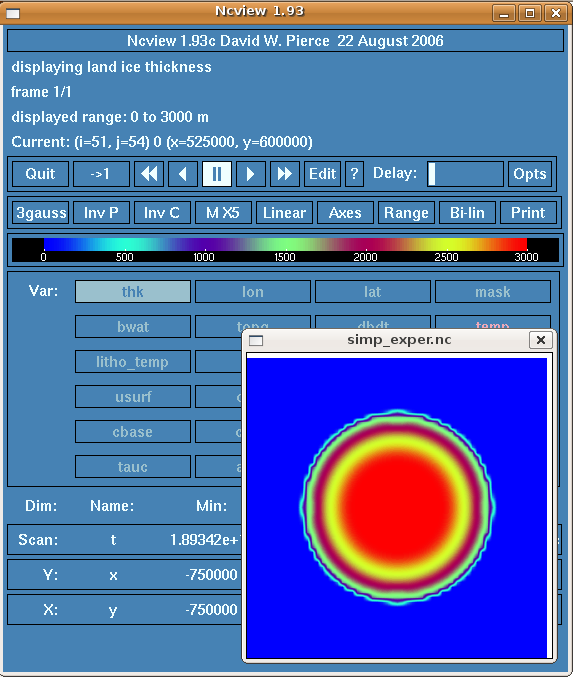
\includegraphics[height=3.5in,keepaspectratio=true]{eisIIA_ncviewshot}
\caption{\texttt{ncview} shows an intermediate stage of an EISMINT II experiment A run.}
\label{fig:ncviewshot}
\end{figure}

Another way to view the output file is graphically.  One of the most convenient tools is \verb|ncview|; see Table \ref{tab:NetCDFview}.  Running ncview on the output file (\verb|ncview simp_exper.nc|) and viewing the ``\t{thk}'' variable gives a figure like \ref{fig:ncviewshot}.

Alternatively, one can use PISM's ``diagnostic viewers'' for a time-dependent view of the evolving modeled ice sheet.  Note this requires X Windows:\index{pisms}\pismoptionindex{eisII}\pismoptionindex{d}

\begin{verbatim}
$ pisms -eisII A -i simp_exper.nc -y 1000 -view_map thk \
        -view_slice temp -slice_level 0 -view_sounding temp
\end{verbatim}
Three figures should appear and be refreshed at each time step.  One figure is a map-plane view of thickness, another is a map-plane view of the basal temperature in Kelvin, and the third is a graph of temperature versus height above the bedrock.  When the full 200,000 year run finishes, one may watch its evolving, though essentially steady, state.  A view that includes the ice flow speed is:
\begin{verbatim}
$ pisms -eisII A -i simp_exper.nc -y 1000 -view_map thk,cbar \
        -view_slice temp -slice_level 0 -view_sounding temp
\end{verbatim}
for example.  Figure \ref{fig:screenshot} will appear.

\begin{figure}[ht]
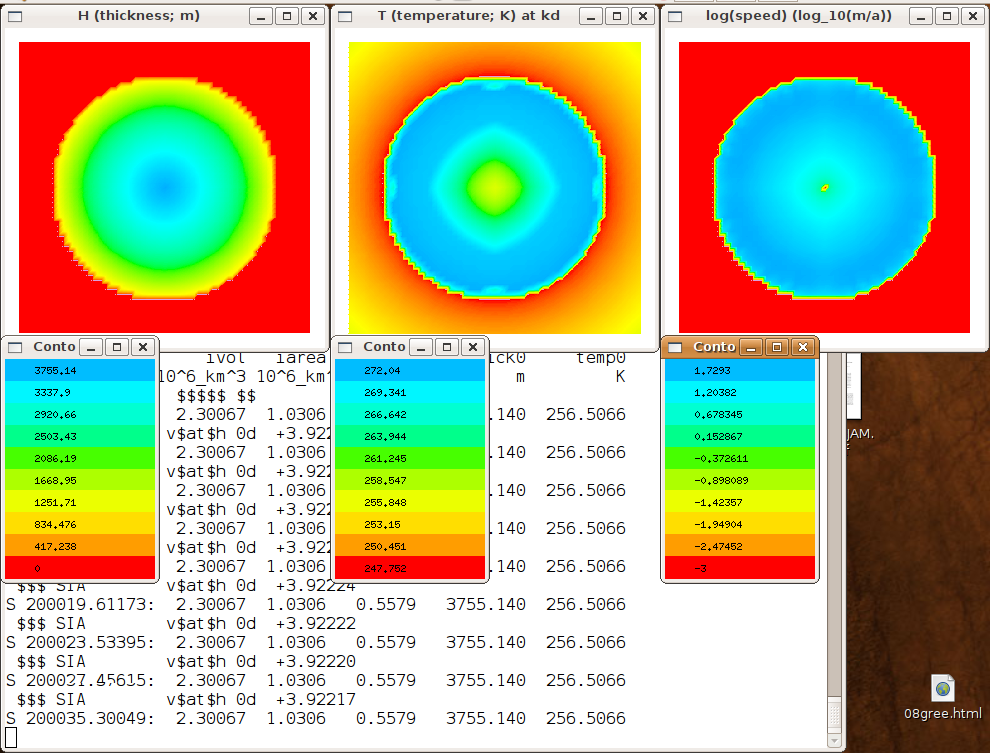
\includegraphics[height=3.5in,keepaspectratio=true]{eisIIAshot}
\caption{Screenshot of diagnostic figures for an EISMINT II experiment A run.}
\label{fig:screenshot}
\end{figure}

As shown by the ``\verb|-view_map|'', ``\verb|-view_slice|'' and ``\verb|-view_sounding|'' options above, it is possible to monitor PISM's model state during the run; see section \ref{sec:diagnostic-viewers} for more. These viewers are updated at each time step and are not used for runs in batch mode or where efficiency is needed.  (As they work under Xwindows, MPI must be told how to send data to the window, so PISM options are usually followed by ``\verb|-display :0|''\pismoptionindex{display} when PISM is run under MPI and runtime viewers are needed.)


\subsection{PISM's standard output}   As seen already, at each time step PISM shows a summary\index{PISM!standard output summary of each time step} of the model state using a few numbers and some single character flags.  The format of the summary is partly explained by two lines near the beginning of the run:

\small\begin{quote}
\begin{verbatim}
P         YEAR:     ivol   iarea    meltf     thick0     temp0
U        years 10^6_km^3 10^6_km^2 (none)          m         K
\end{verbatim}
\end{quote}\normalsize

The ``\t{P}'' line is the prototype for the summary which appears at each time step.  The ``\t{U}'' line gives units for this summary.  From then on, the ``\t{S}'' lines give values for the quantities specified by the  ``\t{P}'' and ``\t{U}'' lines.

The EISMINT II runs above illustrate how the time-stepping in PISM adapts in order to maintain stability for its (mostly) explicit methods.  At the beginning of the EISMINT II run, for instance, the ice has small thickness so the time step is 60 years, simply because that is the default maximum time step.  Later in that run, after about 5000 years, the time step is made smaller because the flow is faster.

After the year, the next three entries in the summary report the volume of the ice in $10^6 \,\text{km}^3$, the area covered by the ice in $10^6\,\text{km}^2$, and the basal melt fraction, that is, the fraction of the ice area where the basal temperature is at the pressure-melting temperature.  This melted-base-fraction is a pure number without units.  The next two columns ``\texttt{thick0}'' and ``\texttt{temp0}'' are values at the center of the computational domain of the map plane, namely the ice thickness in meters and the absolute temperature of the ice at its base, in Kelvin.  These five numbers are the ones reported in the tables in \cite{EISMINT00}, which explains why they are the default quantities for reporting to standard output.  For more on the EISMINT II experiments see section \ref{sect:simp}.

The summary of the model state can be made more verbose by using the option \verb|-verbose|.  

In addition to the ``\t{S}'' lines, there are lines, starting with a space character, which give flags, both cryptic and compact, describing the PISM model choices made at each time step.  Most of these relate to decisions of the adaptive time-stepping scheme.  That scheme is described in subsection \ref{subsect:adapt}

If the standard output from PISM is saved in a text file then it can always be converted to a NetCDF file with corresponding time series.  For the 200,000 year run above,

\verb|$ series.py -f out.eisIIA -o ser.eisIIA.nc|

\verb|$ ncview ser.eisIIA.nc|

A look at these time series shows the convergence to equilibrium of this non-sliding thermomechanically coupled modeled ice sheet.  We see, characteristically, that there is a longer relaxation time for temperature at the base of the ice than for any geometric quantity (volume, area, thickness).

\subsection{Handling NetCDF files}\label{subsect:nctoolsintro}  At a trivial level, PISM is just a program which takes a NetCDF file as input, does some computation, and produces a NetCDF file as output.  (An exception is that \verb|pisms| knows formulas to initialize EISMINT II experiments, for example.)  The user is in charge of creating NetCDF input files containing data on ice sheets worth modeling\footnote{See the section \ref{sec:bootstrapping-format} and table \ref{tab:modelhierarchy} for a hint about data necessary for modeling.}, and extracting some meaning from the NetCDF output files.

The most basic tools for converting NetCDF files to and from a standard text representation are called \verb|ncdump| and \verb|ncgen|.  A glance at Unix \verb|man| pages for these tools might be wise at this time.

As suggested earlier, we regularly use \verb|ncview| to look at NetCDF files.  The NetCDF tools most frequently used by the PISM developers are shown in Table \ref{tab:NetCDFview}.  This website gives additional NetCDF-related tools:

\centerline{ \href{http://www.unidata.ucar.edu/software/netcdf/docs/software.html}{\t{www.unidata.ucar.edu/software/netcdf/docs/software.html}} } 

\begin{table}[ht]
\caption{Some tools for viewing and modifying NetCDF files.}\label{tab:NetCDFview} 
\small
\begin{tabular}{@{}llll}\hline
\textbf{Tool} & \textbf{Site} & \textbf{Function}\\ \hline
\verb|ncdump| & \emph{included with any NetCDF distribution} & dump binary NetCDF as \texttt{.cdl} (text) file \\
\verb|ncgen| & \emph{included with any NetCDF distribution} & convert \texttt{.cdl} file to binary NetCDF \\
\verb|ncview|\index{ncview} & \href{http://meteora.ucsd.edu/~pierce/ncview_home_page.html}{\texttt{meteora.ucsd.edu/$\sim$pierce}} & quick graphical view \\
IDV & \href{http://www.unidata.ucar.edu/software/idv/}{\t{www.unidata.ucar.edu/software/idv/}} & more complete visualization \\
Paraview & \href{http://www.paraview.org}{\t{www.paraview.org}} & powerful open-source parallel visualization \\
NCL &  \href{http://www.ncl.ucar.edu}{\t{www.ncl.ucar.edu}} & NCAR Command Language, open-source\\
PyNGL &  \href{http://www.pyngl.ucar.edu}{\t{www.pyngl.ucar.edu}} & Python version of NCL, open-source\\
VisIt & \href{http://visit.llnl.gov}{\t{visit.llnl.gov}} & advanced parallel visualization \\
NCO\index{NCO (NetCDF Operators)} & \href{http://nco.sourceforge.net/}{\t{nco.sourceforge.net/}} & ``NetCDF Operators'': manipulations \\
\quad  & & \quad at command line
\end{tabular}
\normalsize
\end{table}


%%% Local Variables: 
%%% mode: latex
%%% TeX-master: "manual"
%%% End: 

